\documentclass[11pt,letterpaper]{article}

% Month 2 Progress Report (main document).
% The Month 1 report is archived in archive/month1_report.tex (+ archive/month1_report.pdf).
% Figures in figures/month2 and table bodies in tables/month2 are generated by
% month2_sources/make_figures.py from the published tables copied in month2_sources/data.

\usepackage[utf8]{inputenc}
\usepackage[T1]{fontenc}
\usepackage{lmodern}
\usepackage[margin=1in]{geometry}
\usepackage{amsmath,amssymb}
\usepackage{booktabs}
\usepackage{graphicx}
\usepackage{float}
\usepackage{xcolor}
\usepackage{caption}
\usepackage{array}
\usepackage{tabularx}
\usepackage[hidelinks]{hyperref}

\hypersetup{colorlinks=true,linkcolor=blue!50!black,citecolor=blue!50!black,urlcolor=blue!50!black}
\captionsetup{font=small,labelfont=bf}
\setlength{\parskip}{0.45em}
\setlength{\parindent}{0pt}
\makeatletter
\def\@listi{\leftmargin\leftmargini\topsep 2pt\parsep 0pt\partopsep 0pt\itemsep 2pt}\let\@listI\@listi
\def\@listii{\leftmargin\leftmarginii\topsep 1pt\parsep 0pt\partopsep 0pt\itemsep 1pt}
\newcommand{\tabinput}[1]{\@@input #1 }
\makeatother
\renewcommand{\arraystretch}{1.08}

\newcommand{\K}{\,\mathrm{K}}
\newcommand{\pon}{with~$\mathbf{p}$}
\newcommand{\poff}{without~$\mathbf{p}$}
\newcommand{\NH}{\text{NH}_3}
\newcommand{\cond}[2]{#1\%\,$\NH$, $\phi{=}#2$}
\newcommand{\keybox}[1]{\par\smallskip\noindent\fcolorbox{black!35}{black!3}{\parbox{\dimexpr\linewidth-2\fboxsep-2\fboxrule\relax}{\small #1}}\par\smallskip}

\title{\textbf{Month 2 Progress Report}\\[0.3em]
\large Temperature-Free Reconstruction, Few-Sensor Corrections and Temperature-Input Training\\[0.5em]
\normalsize Neural Reconstruction of Hidden Temperature Fields from Sparse Observations in Turbulent Combustion}
\author{\textbf{Enrico Bontempi}\\
M.Sc.\ Thesis Project --- Deng Energy and Nanotechnology Group, MIT}
\date{November 2026}

\begin{document}
\maketitle

\begin{abstract}
\noindent
This report describes the Month~2 experiments on reconstructing an instantaneous $128\times128$ temperature field of a turbulent $\NH/\text{CH}_4$/air flame from sparse observations of planar velocity. We studied three questions in sequence. (1)~Without any temperature measurement, how well do a masked U-Net and an adapted GLU reconstruct the field from 5\% of the velocity vectors, with and without the operating parameters $\mathbf{p}=(\NH\%,\phi)$ as additional inputs (ammonia percentage in the fuel blend and equivalence ratio), and how much does the amount of training data matter? (2)~If a few ideal point temperatures become available at inference, how much can they correct a frozen temperature-free prediction? (3)~Does a network that receives those temperatures directly as input do better than such a post hoc correction? Both neural families have 1.6 to 2.5 times lower error than the best linear baseline (GappyPOD). The U-Net has the lower structural error and the GLU the more accurate thermal level. A median offset computed from four or more temperature sites removes most of the remaining level error but leaves the spatial structure unchanged, and the temperature-input training gives a measurable benefit in only one of four configurations. All evidence comes from three validation conditions that were also used for model selection. The report closes with three possible directions for Month~3, presented for discussion.
\end{abstract}

\clearpage
{\setcounter{tocdepth}{1}\tableofcontents}
\bigskip

%======================================================================
\section{Executive summary}
\label{sec:summary}

\textbf{Question.} The thesis asks how accurately an instantaneous temperature field can be reconstructed from incomplete observations of other variables, and how this changes for operating conditions excluded from training. Month~1 established the data split, the error decomposition $\text{RMSE}^2=\text{bias}^2+\text{centered RMSE}^2$ (per frame) and linear baselines. Month~2 trained the first neural reconstructors and examined what limits them: the spatial \emph{structure} of the flame (jets, shear layers) or the overall thermal \emph{level}, and whether a few temperature measurements can fix either.

\textbf{Input convention.} Throughout this report, $\mathbf{p}=(\NH\%,\phi)$ denotes the ammonia percentage in the fuel blend and the equivalence ratio. The labels \texttt{p\_on} (\pon) and \texttt{p\_off} (\poff) mean that \emph{both} operating parameters are supplied as model inputs or excluded from the inputs, respectively. They do not indicate whether temperature observations are available; that is specified separately by $K$.

\textbf{What we did.} We ran three experiments on the same data and observation protocol (Section~\ref{sec:protocol}). We first studied training-data quantity (19, 38 and 149 snapshots per training condition). We then compared a masked U-Net and an adapted GLU, each with and without $\mathbf{p}$, over three training seeds, with no temperature input. Next, we corrected the frozen predictions with $K\in\{0,1,4,9,16,32\}$ ideal temperature sites. Finally, we trained twelve new networks that receive those $K$ temperatures and their positions as input.

\textbf{Main results.} All values are macro RMSE in kelvin on the three validation (VAL) conditions, mean over three training seeds, with 5\% observed velocity and the best checkpoint.
\begin{enumerate}
  \item \textbf{More snapshots help, mainly in structure.} Going from 38 to 149 training snapshots per condition lowers the VAL error of the U-Net from $42.4$ to $38.7\K$ (\pon) and from $42.9$ to $39.8\K$ (\poff), and the error on later frames of the training conditions by $5$--$15\K$ (single seed). The jets improve most. A cold level bias on one VAL condition remains (Section~\ref{sec:data}).
  \item \textbf{Neural reconstruction is far more accurate than the baselines, with different strengths per family.} Full-field VAL RMSE is $39.7$ (U-Net \pon), $40.6$ (U-Net \poff), $42.7$ (GLU \pon) and $44.5\K$ (GLU \poff), against $70.6\K$ for GappyPOD and $87.7\K$ for the parametric mean field. The U-Net has clearly lower structural error (centered RMSE $34.4$--$35.1$ vs $40.9$--$41.0\K$) and lower error on later frames of training conditions. The GLU has a more accurate level (signed bias $+0.1$ to $+1.8\K$ vs about $-8\K$) and degrades less at 1\% velocity. Seed ranges overlap in RMSE. Replacing the observed velocities with those of another snapshot raises the VAL error by $52$--$64\K$, so the predictions depend on the observed instant (Section~\ref{sec:free}).
  \item \textbf{A median offset from $K\ge4$ temperatures corrects the level, not the structure.} For the U-Net \pon, the median of the residuals at the observed sites lowers the error from $39.70$ to $34.85\K$ at $K{=}4$ and $34.54\K$ at $K{=}32$, close to the diagnostic limit of a perfect uniform shift ($34.38\K$). The centered RMSE and the error in the cold jets do not improve. With one site, the average error rises strongly ($68.5\K$). This average is dominated by one of the three layouts, whose single site falls inside a cold jet. On later frames of training conditions, where the level is already accurate, the median gives little or no gain at small $K$ (Section~\ref{sec:correction}).
  \item \textbf{Temperatures as network input helped only one configuration measurably.} Compared with the same model evaluated without temperatures ($K{=}0$), the gain at $K{=}32$ is $\le0.13\K$ for three configurations. The GLU \poff\ gains $2.94\K$ on VAL and $2.26\K$ on later frames of training conditions, partly structural. On VAL at $K\ge4$, the free model plus median is lower on average in all four configurations, narrowly for the GLU \poff\ (Section~\ref{sec:assisted}).
\end{enumerate}

\textbf{Main limits.} The three VAL conditions were used to select checkpoints, adjust the learning rate and stop training, and the median estimator was chosen after observing a failure of the mean on VAL. VAL numbers are therefore development evidence, not an independent confirmation. Temperatures are ideal numerical samples without noise. Training frames are temporally correlated. No TEST data were used in Month~2 experiments. The TEST conditions were already examined with the Month~1 baselines.

\textbf{Provisional operating reference.} For further work, we propose to use the U-Net \pon\ trained without temperatures at 5\% velocity as the working reference (U-Net \poff\ when $\mathbf{p}$ is unknown), and the same model plus the median offset when $K\ge4$ ideal temperatures are available. This is a development choice made after seeing the results, not a definitive model. The GLU and the temperature-input models remain documented alternatives.

\textbf{For discussion.} Section~\ref{sec:month3} presents three possible directions for Month~3. They are a jet-weighted training loss for the temperature-free task, a check of whether the level error generalizes to further held-out conditions, and a spatial assimilation of temperature residuals on a frozen network. They are compatible with each other and could be run as one bounded, ordered program. No direction has been chosen.

%======================================================================
\section{Objective and progress since Month 1}
\label{sec:objective}

The engineering motivation is combustion diagnostics with limited measurement access. Planar velocity can be measured optically, often with gaps, whereas temperature is typically available only at a few intrusive points. The thesis therefore studies the reconstruction of a single instantaneous temperature field from incomplete observations and asks how the reconstruction degrades when the observations or the operating condition change. The dataset is the numerical LES combustion set of \textit{RealPDEBench}~\cite{hu2026realpdebench}: 30 operating conditions of a swirl-stabilized $\NH/\text{CH}_4$/air burner on a $128\times128$ diametral slice. Two cold reactant jets enter from the right boundary around a hot recirculation zone.

Month~1 produced three results that shaped Month~2. Knowing $\mathbf{p}$ fixes much of the mean temperature level. The main difficulty is the instantaneous structure along the jets and the flame brush. Linear GappyPOD~\cite{everson1995gappy} leaves a large gap to the projection of the true field onto the same basis. The Month~1 plan proposed a dense diagnostic, a sparse GLU-type model~\cite{wang2026glu} compared with a masked U-Net, and a residual treatment of a few temperature sensors.

The following protocol choices were fixed at the start of Month~2 and are kept throughout this report: single-frame input, planar two-component velocity $(v_i,v_j)$, and temperature as the supervised target only. A dense diagnostic was run first, with full velocity and seed~0 on 38 frames per condition. A U-Net reached $26.9\K$ VAL RMSE \pon\ and $39.7\K$ \poff, against $70.5\K$ for dense GappyPOD \pon. Exchanging the velocity field with that of another snapshot raised the error by $63$--$70\K$. This showed that single-frame velocity carries substantial instantaneous information when it is fully observed. These dense values are not comparable with the sparse results below, which use less information and more training data.

Month~2 then examined four factors, in this order:
\begin{itemize}
  \item \textbf{Structure versus level.} An earlier diagnostic on 38-frame models showed that part of the VAL error is a uniform level offset. On \cond{40}{0.90}, a U-Net with a good flame shape lost most of its hot region because its whole field was about $29\K$ too cold. Errors of this kind and errors in the jets call for different remedies.
  \item \textbf{Data quantity.} Before comparing architectures, we checked whether the models were limited by the number of training snapshots.
  \item \textbf{Architecture and operating parameters.} U-Net versus GLU, each with and without $\mathbf{p}$, over three seeds.
  \item \textbf{Thermal information.} How much a few temperature measurements add, first as a correction of a frozen prediction and then as network input. The proposal foresaw this temperature-assisted setting as a separate track and as a fallback if velocity alone proved insufficient.
\end{itemize}

%======================================================================
\section{Experimental protocol}
\label{sec:protocol}

This section gives what is needed to read the results. Appendix~\ref{app:protocol} lists the full definitions.

\textbf{Data and roles.} The operating-condition split of Month~1 is unchanged: 20 TRAIN, 3 VAL, 3 interpolation-TEST and 4 extrapolation-TEST conditions. Results use three evaluation roles:
\begin{itemize}
  \item \textbf{VAL} (123 frames): the three held-out conditions \cond{0}{1.05}, \cond{20}{1.10} and \cond{40}{0.90}, 41 frames each over the full trajectory.
  \item \textbf{seen} (220 frames): frames 1600--2000 of the 20 TRAIN conditions, separated by at least 120 frames from all training frames. These are new snapshots of training conditions, not new conditions.
  \item \textbf{fit reference} (760 frames): a subset of the training frames, used only to measure fitting.
\end{itemize}
All main models are trained on 149 frames per TRAIN condition (2980 frames, indices 0--1480 every 10 frames). These frames are strongly correlated in time, so 2980 frames are not 2980 independent samples. The fit-only normalisation computed on the 760 reference frames was kept frozen for every pool.

\textbf{Observations.} The models see the two in-plane velocity components at 5\% of the grid (819 sites), plus pixel coordinates. The \pon\ variants also see $\mathbf{p}$. Training masks are resampled. Evaluation uses three fixed mask replicas, nested so that 1\% $\subset$ 5\% $\subset$ 20\%. The 1\% and 20\% levels test generalization away from the 5\% training density. For the temperature experiments, three fixed layouts of 32 sites were drawn at random from the grid without using any temperature information (Figure~\ref{fig:layouts}). They are nested so that the first $K$ sites form the layout for each $K$. Layout $r$ is always paired with velocity mask replica $r$, so the variability across the three pairs mixes the two sources. Temperatures are exact simulation values without noise.

\begin{figure}[!htb]
  \centering
  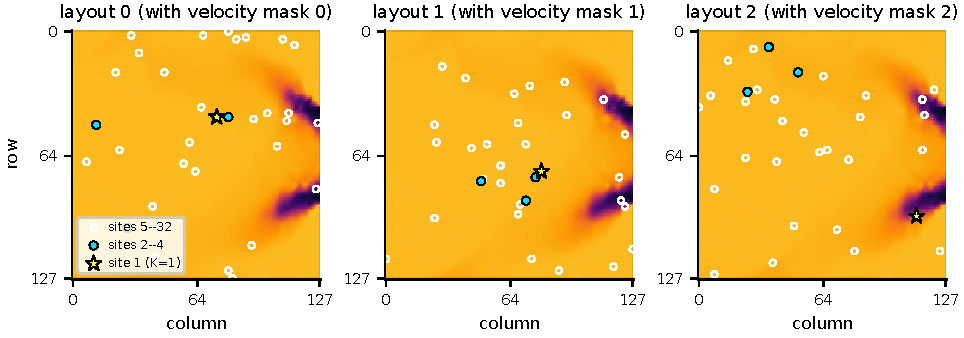
\includegraphics[width=\textwidth]{figures/month2/anchor_layouts.pdf}
  \caption{The three nested temperature-site layouts used in Experiments~2 and~3, drawn over one VAL snapshot (\cond{0}{1.05}, frame 1000, true temperature, colour scale $208$--$2652\K$) for orientation only. Star: the single site used at $K{=}1$. Cyan: sites 2--4 ($K{=}4$). White circles: sites 5--32. Sites are fixed for every frame and condition. In layout~2 the first site (row 95, column 112) lies in the lower cold jet. The 5\% velocity sites are not shown.}
  \label{fig:layouts}
\end{figure}

\textbf{Models.} Both families output the full temperature field and are trained with a uniform mean-squared error on all pixels.
\begin{itemize}
  \item The \textbf{masked U-Net}~\cite{ronneberger2015unet} (4.90\,M parameters) takes the velocity values with an explicit observation mask, coordinates and, \pon, two constant channels for $\mathbf{p}$. Unobserved velocities are not presented as physical zeros.
  \item The \textbf{adapted GLU} (1.15\,M parameters) is a deterministic version of the laboratory model~\cite{wang2026glu}. It encodes each observed site as a token (position and velocity), uses a global token and local $k$-nearest-neighbour fusion, and adds $\mathbf{p}$ through a learned projection. The uncertainty head and temporal components of the original are not used.
\end{itemize}
The two families differ in capacity and implementation, so the comparison is between two specific recipes, not between architecture classes.

\textbf{Training and checkpoints.} Both families use the same recipe: AdamW, effective batch 8, a plateau learning-rate scheduler on the VAL error, evaluation every 10 epochs, and early stopping after at least 200 epochs and 15 evaluations without 0.1\% relative improvement. All runs in this report stopped by this plateau criterion. We report two checkpoints:
\begin{itemize}
  \item \textbf{best}: the first minimum of the VAL error at 5\%;
  \item \textbf{last}: the checkpoint at the early stop.
\end{itemize}
Selecting on VAL makes VAL results optimistic. Earlier models showed a gap of $1$--$4\K$ between the minimum over three VAL conditions and a leave-one-condition-out estimate. Each configuration is trained with seeds 0, 1 and 2. Seeds are training repetitions, whereas the three mask replicas are repetitions of the observations. They are averaged separately and never counted as independent trainings.

\textbf{Metrics.} The \emph{macro RMSE} is the per-frame RMSE in kelvin, averaged over the frames of each condition, then over conditions, then over mask replicas. We also report the signed \emph{bias} (mean of predicted minus true), the mean per-frame $|\text{bias}|$ and the \emph{centered RMSE} (RMSE after removing each frame's own bias). The identity $\text{RMSE}^2=\text{bias}^2+\text{centered}^2$ holds per frame, not after averaging, so we never derive one macro from the others. Regional metrics are the RMSE in the \emph{cold jets} ($T<1800\K$, about 7\% of the VAL area) and in the \emph{hot region} ($T\ge2100\K$), and the intersection over union (IoU) of the predicted and true hot regions. For the temperature experiments, the primary domain is the \textbf{common domain}: the grid minus all 32 sites of the layout (16352 pixels), identical for every $K$. Unless stated otherwise, RMSE values in Sections~\ref{sec:correction}--\ref{sec:assisted} are common-domain values. Free-model values on this domain differ from full-field values by less than $0.05\K$.

\begin{table}[!htb]
\centering
\caption{The three Month~2 experiments. All use the 149-frame training pool, 5\% training velocity, seeds 0/1/2, VAL and seen roles, and no TEST data.}
\label{tab:design}
\small
\begin{tabularx}{\textwidth}{>{\raggedright\arraybackslash}p{2.6cm}>{\raggedright\arraybackslash}X>{\raggedright\arraybackslash}X>{\raggedright\arraybackslash}X}
\toprule
 & \textbf{1. Temperature-free} & \textbf{2. Post hoc correction} & \textbf{3. Temperature as input} \\
\midrule
Question & What does sparse velocity alone give, per family and with/without $\mathbf{p}$? & How much do $K$ ideal temperatures correct a frozen prediction? & Does learning to use the temperatures help beyond a correction? \\
Models & U-Net, GLU $\times$ \pon/\poff\ $\times$ 3 seeds: 12 runs (10 new, 2 reused) & The 12 frozen models of Exp.~1, plus baselines & 12 new trainings, same families, $\mathbf{p}$ settings and seeds \\
Temperature input & none & $K\in\{0,1,4,9,16,32\}$ residuals, used only after prediction & same $K$ values and sites as input; $K$ drawn per batch in training \\
Evaluation & 1/5/20\% velocity; snapshot swap & common domain, four estimators + oracle & common domain, compared with own $K{=}0$ \\
Selection & first VAL minimum at 5\% & none (no estimator selected) & first minimum of VAL error averaged over the six $K$ \\
\bottomrule
\end{tabularx}
\end{table}

%======================================================================
\section{Temperature-free reconstruction}
\label{sec:free}

\subsection{How much training data is needed?}
\label{sec:data}

Before comparing families, we checked whether the U-Net was limited by the number of training snapshots. Three nested pools were used: 19, 38 and 149 frames per TRAIN condition. Training was otherwise identical, with the same number of optimizer updates per epoch. This study used seed~0 only, plus a second seed at 38 frames.

\begin{figure}[!htb]
  \centering
  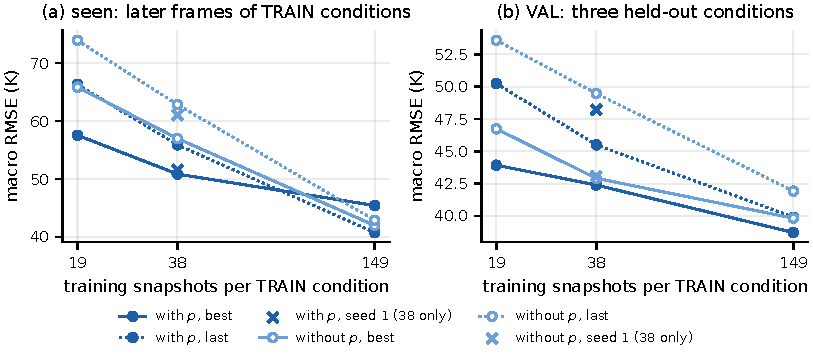
\includegraphics[width=0.82\textwidth]{figures/month2/data_quantity.pdf}
  \caption{U-Net macro RMSE versus training snapshots per TRAIN condition, 5\% velocity, mean of three mask replicas, seed~0. Solid lines: best checkpoint (first VAL minimum); dotted lines: last checkpoint. Crosses: a second training seed at 38 frames. (a)~seen role; (b)~VAL role.}
  \label{fig:data}
\end{figure}

Figure~\ref{fig:data} shows that more snapshots help on both roles. On VAL, going from 38 to 149 frames per condition lowers the error at the best checkpoint from $42.39$ to $38.71\K$ (\pon) and from $42.92$ to $39.82\K$ (\poff), in all three conditions. The gain is mostly structural. Centered RMSE falls by about $3\K$ at the best checkpoint and $7\K$ at the last one, and the jet RMSE by $12$--$13\K$ and $22\K$ respectively. Overfitting after the minimum is also much weaker. With 38 frames, the last checkpoint was $3$--$7\K$ worse than the best on VAL. With 149 frames, the gap shrinks to $1$--$2\K$, and on seen frames the last checkpoint of the model \pon\ is even better than its best.

Two observations limit this result. First, more data did not remove the cold level bias on \cond{40}{0.90}, which stayed between $-22$ and $-26\K$ for the \pon\ model. Second, the two seeds at 38 frames differed by $5.8\K$ on VAL (\pon). This difference came entirely from the level on that same condition, while the structural errors were nearly equal. A single seed can therefore move VAL averages by several kelvin, which is why all later experiments use three seeds. We adopted the 149-frame pool for all further work.

\subsection{U-Net and GLU, with and without operating parameters}
\label{sec:families}

Table~\ref{tab:free} and Figure~\ref{fig:free} summarize the twelve temperature-free models. Ten were newly trained and two U-Net seed-0 runs were reused from the data-quantity study after verifying their provenance.

\begin{table}[!htb]
\centering
\caption{Temperature-free reconstruction at 5\% velocity, best checkpoint. Neural rows: mean over three seeds, with the seed range in brackets. Each seed value is itself the mean of three mask replicas. Baselines are fitted once on the same 149-frame pool. Errors in K. IoU refers to the hot region $T\ge2100\K$. seen = later frames of the TRAIN conditions.}
\label{tab:free}
\footnotesize
\setlength{\tabcolsep}{3.2pt}
\begin{tabular}{llrrrrrrrr}
\toprule
 & & \multicolumn{6}{c}{\textbf{VAL} (3 held-out conditions)} & \multicolumn{2}{c}{\textbf{seen}} \\
\cmidrule(lr){3-8}\cmidrule(lr){9-10}
Model & $\mathbf{p}$ & RMSE & centered & $|$bias$|$ & bias & jets & IoU & RMSE & centered \\
\midrule
\tabinput{tables/month2/free_summary.tex}
\bottomrule
\end{tabular}
\end{table}

\begin{figure}[!htb]
  \centering
  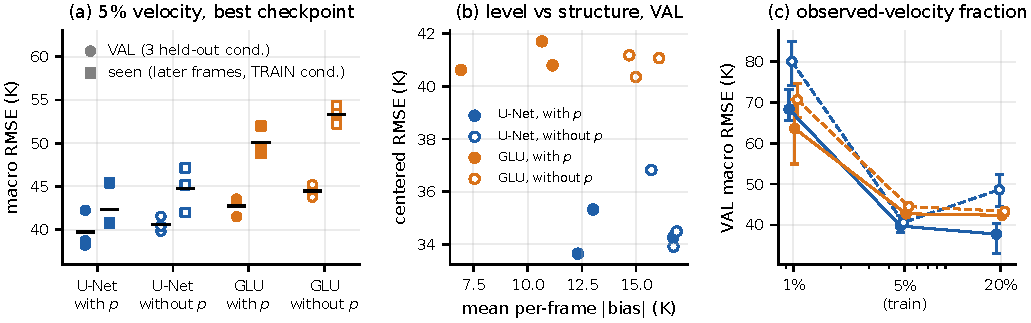
\includegraphics[width=\textwidth]{figures/month2/free_comparison.pdf}
  \caption{Temperature-free models, best checkpoint. (a)~Macro RMSE at 5\% velocity. Each marker is one training seed (mean of three mask replicas); bars mark the mean over seeds. Filled markers: \pon; open markers: \poff. (b)~VAL centered RMSE (structure) against mean per-frame $|\text{bias}|$ (level), one point per seed. (c)~VAL RMSE when the models, trained at 5\%, are evaluated at 1\% and 20\% observed velocity. Points show the seed mean and bars the seed range.}
  \label{fig:free}
\end{figure}

\textbf{Both families are far better than the baselines.} On VAL, the neural models reach $39.7$--$44.5\K$. GappyPOD with $\mathbf{p}$ reaches $70.6\K$, the parametric mean field $87.7\K$ and the global mean $139.6\K$. On seen frames the gap is wider: $42$--$53\K$ against $108\K$ for GappyPOD.

\textbf{The two families have different strengths.}
\begin{itemize}
  \item \emph{Structure (U-Net better).} The U-Net reconstructs the flame structure better. Its VAL centered RMSE is $34.4$--$35.1\K$ against $40.9$--$41.0\K$ for the GLU, consistently over seeds. Its jet RMSE is $113\K$ against $131$--$137\K$. On seen frames its RMSE is $42.3$--$44.8\K$ against $50.1$--$53.3\K$.
  \item \emph{Level (GLU better).} The GLU has the more accurate level. Its signed VAL bias is $+1.8\K$ (\pon) and $+0.1\K$ (\poff), against $-7.8$ and $-8.3\K$ for the U-Net. With $\mathbf{p}$, its mean $|\text{bias}|$ is $9.6\K$ against $14.0\K$, and its hot-region IoU is higher ($0.95$ against $0.80$).
\end{itemize}
The overall RMSE ranking favours the U-Net, but the seed ranges overlap. For example, the U-Net \pon\ seed~1 ($42.2\K$) is worse than the GLU \pon\ seed~1 ($41.5\K$). The U-Net \pon\ is also the least stable configuration across seeds, with a VAL range of $4.0\K$.

\textbf{Operating parameters help mainly the level, and only modestly.} Adding $\mathbf{p}$ lowers the VAL RMSE by $0.9\K$ (U-Net) and $1.8\K$ (GLU). For the GLU the gain is entirely in the level (its centered RMSE does not improve). For the U-Net it is split between level and structure. With 149 frames per condition, the models \poff\ already infer much of the regime from velocity alone.

\textbf{Observed-velocity fraction.} All models were trained at 5\% only. At 1\% the error rises to $63.6$--$80.0\K$ on VAL. The GLU degrades least ($63.6\K$ \pon), and the U-Net \poff\ degrades most ($80.0\K$, with a $-39\K$ bias). At 20\%, the U-Net \poff\ becomes \emph{worse} than at 5\% ($48.6$ vs $40.6\K$, bias $+7.5\K$), while the GLU stays nearly flat. On seen frames, the U-Net \pon\ also worsens at 20\% ($47.1$ vs $42.3\K$). One possible explanation is that the U-Net sees the observation mask as an input channel whose statistics change with density. We have not tested this hypothesis. These curves describe generalization from a single training density. They are not an optimal sensor-count curve.

\textbf{Dependence on the observed snapshot.} We replaced the velocities at the observed sites by those of a different snapshot (same sites, coordinates, $\mathbf{p}$ and target). The VAL error then rises from $39$--$45\K$ to $97$--$101\K$, an increase of $52$--$64\K$. This is close to the error obtained by predicting the donor snapshot's own temperature ($97.4\K$). On seen frames it rises by $93$--$110\K$. Every run, in every condition, gets worse. The models therefore use the instantaneous velocity pattern rather than only the condition or the mask. This is a sensitivity test, not a proof of a physical causal mechanism.

\textbf{Checkpoint and fitting.} The U-Net reaches its VAL minimum early (epochs 90--260) and keeps fitting the training frames afterwards. Its error on the fit-reference frames falls to about $14\K$ at the last checkpoint, while VAL worsens by $1.0$ (\pon) and $2.4\K$ (\poff). The GLU converges more slowly (best epochs 290--650) and fits the training frames less tightly ($43\K$ at best).

\subsection{Structure, level and difficult cases}
\label{sec:cases}

\begin{figure}[!htb]
  \centering
  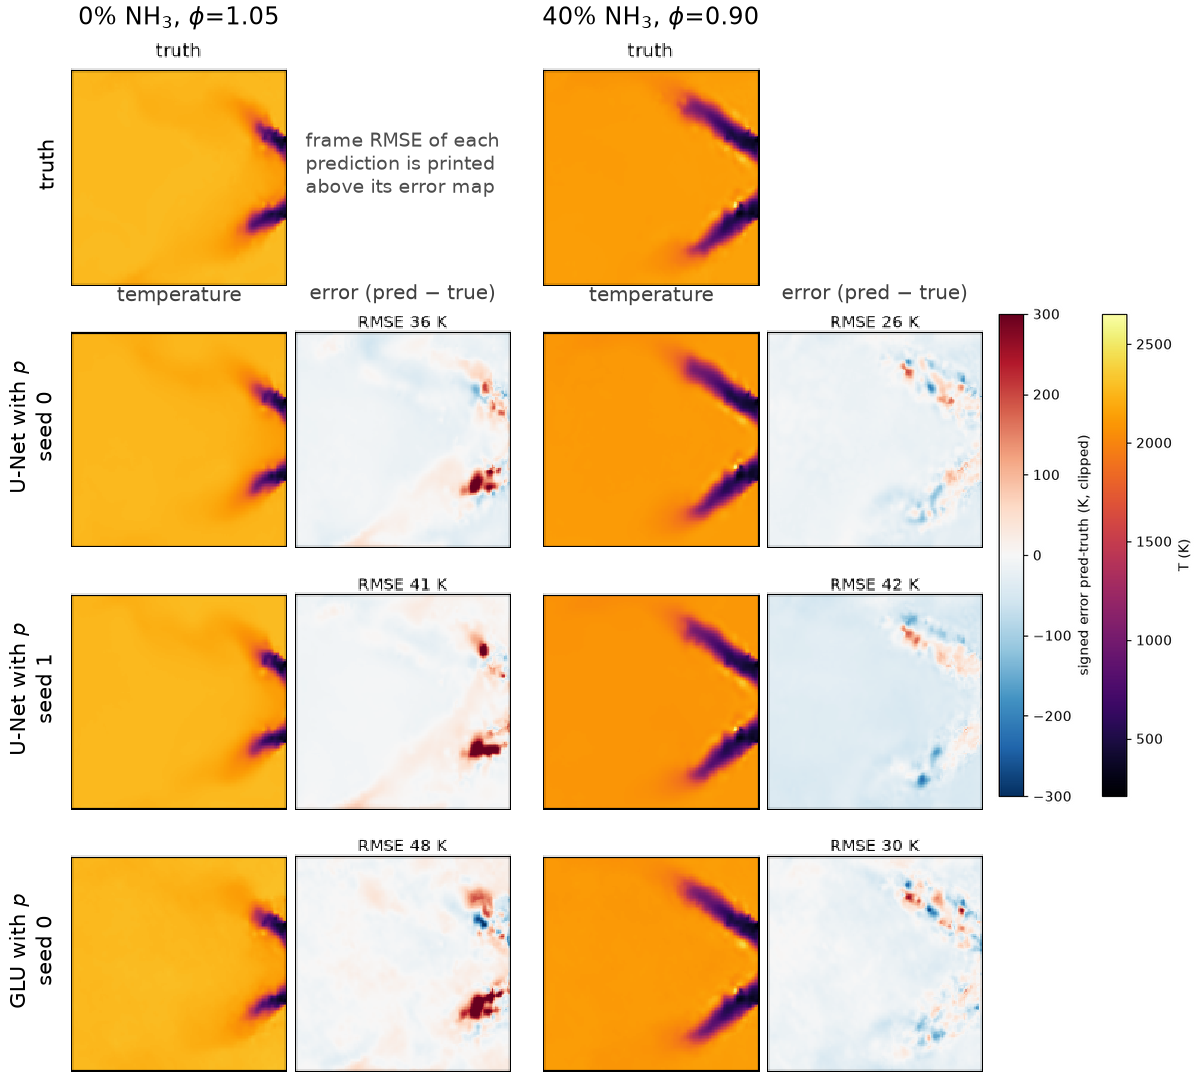
\includegraphics[width=0.94\textwidth]{figures/month2/fields_level_structure.png}
  \caption{One VAL frame (frame 1000) for two conditions, 5\% velocity, mask replica~0, best checkpoints. Left column of each pair: temperature; right column: signed error (prediction minus truth). All panels share the scales $T\in[208,2652]\K$ and error $\pm300\K$. Errors are clipped for display; the largest absolute error over these figures is $720\K$. The frame RMSE is printed above each error map. On \cond{40}{0.90}, the U-Net seed~1 reproduces the flame shape but is uniformly too cold (light blue background). On \cond{0}{1.05}, errors concentrate in the cold jets for all models. The panels are crops of the published comparison figure of all twelve models, without modification of the data.}
  \label{fig:fields}
\end{figure}

\begin{figure}[!htb]
  \centering
  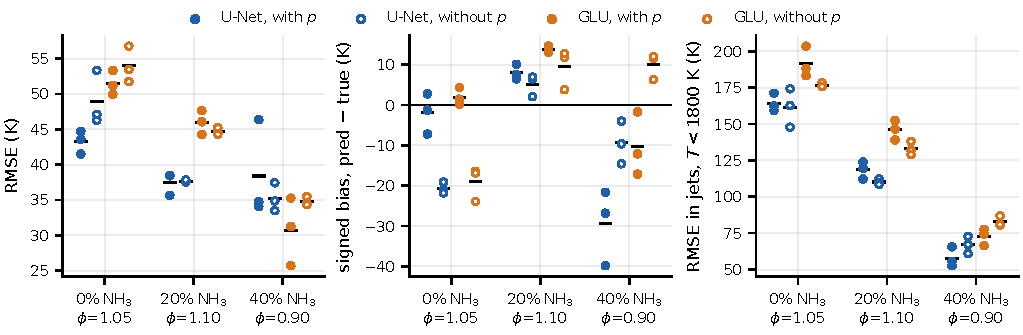
\includegraphics[width=\textwidth]{figures/month2/free_val_conditions.pdf}
  \caption{Temperature-free models per VAL condition, 5\% velocity, best checkpoint. Each marker is one seed (mean of three mask replicas); bars mark the seed mean. Left: RMSE. Centre: signed bias (prediction minus truth). Right: RMSE in the cold jets ($T<1800\K$).}
  \label{fig:valcond}
\end{figure}

The three VAL conditions fail in different ways (Figures~\ref{fig:fields} and~\ref{fig:valcond}; per-condition values in Table~\ref{tab:freecond}):
\begin{itemize}
  \item \textbf{\cond{40}{0.90}: correct structure, wrong level.} This flame has the lowest structural error, but the U-Net \pon\ is too cold by $29.4\K$ on average, with a seed range from $-21.6$ to $-39.8\K$. Because about 78\% of the true field lies above the $2100\K$ threshold, mostly close to it, this offset destroys the hot-region overlap. The IoU falls to $0.43$ on average and to $0.10$ for one seed. The GLU \pon\ has a smaller offset ($-10.3\K$, IoU $0.87$). In Figure~\ref{fig:fields}, the U-Net seed~1 shows the typical pattern: a correct flame with a uniformly blue error map.
  \item \textbf{\cond{0}{1.05}: structural errors in the jets.} This is the hardest condition for 11 of the 12 runs. Jet RMSE reaches $162$--$192\K$, concentrated where the cold jets enter. Without $\mathbf{p}$, both families are also too cold by about $20\K$.
  \item \textbf{\cond{20}{1.10}: U-Net clearly ahead.} The U-Net reaches $37.5\K$, against $44.7$--$46.0\K$ for the GLU, with and without $\mathbf{p}$.
\end{itemize}
These cases motivate the next experiment. A level error can in principle be fixed by a few temperature measurements, whereas a jet error cannot be fixed by a uniform shift.

\keybox{\textbf{Supported.} Sparse single-frame velocity at 5\% supports reconstructions with 1.6 to 2.5 times lower error than GappyPOD and about twice lower than the parametric mean field, and the predictions depend on the observed instant. In the tested recipes, the U-Net has better structure and the GLU better level. More training snapshots improve structure.
\textbf{Uncertain.} Whether the ranking holds for other capacities, densities and conditions; the cause of the U-Net degradation at 20\%; whether the cold bias on \cond{40}{0.90} is systematic for held-out conditions or specific to this case.}

%======================================================================
\section{Correcting frozen predictions with a few temperatures}
\label{sec:correction}

\subsection{Motivation and estimators}

If part of the error is a uniform offset, a few point temperatures could estimate it. Let $\hat T_0$ be the frozen temperature-free prediction and $r_k=T(\mathbf{x}_k)-\hat T_0(\mathbf{x}_k)$ the residuals at the $K$ observed sites. We add a single constant $\delta$ to the whole field, $\hat T=\hat T_0+\delta$, using one of four estimators:
\[
\delta_{\text{mean}}=\tfrac1K\sum_k r_k,\qquad
\delta_{\text{AO}}=\tfrac{1}{K+\tau}\sum_k r_k\ (\tau{=}1),\qquad
\delta_{\text{median}}=\operatorname{median}_k r_k,\qquad
\delta_{\text{oracle}}=\overline{T-\hat T_0}.
\]
The shrunk mean $\delta_{\text{AO}}$ is the Month~1 anchor offset. The oracle shift uses the full true field and serves only as a diagnostic limit for any uniform correction. A uniform shift cannot change the centered RMSE, which we verified to $10^{-13}\K$. At $K{=}1$ the mean and the median coincide.

The median was included because of an earlier diagnostic on 38-frame models. That diagnostic used a fixed $3\times3$ grid of nine sites. Two of its sites lay on the jet edges, where local residuals reach several hundred kelvin. The shrunk mean of the nine residuals then worsened three of four networks on VAL. On the same nine sites, the median brought all of them within $0.5\K$ of the oracle. The median was therefore chosen \emph{after} observing a failure on VAL. Applying it to new models and new random layouts tests the same development data again; it is not an independent validation.

The correction was applied to the best and last checkpoints of all twelve models of Section~\ref{sec:free}, and to the baselines. Comparing different $K$ on the common domain ensures that every $K$ is scored on the same 16352 pixels.

\subsection{Results}

\begin{figure}[!htb]
  \centering
  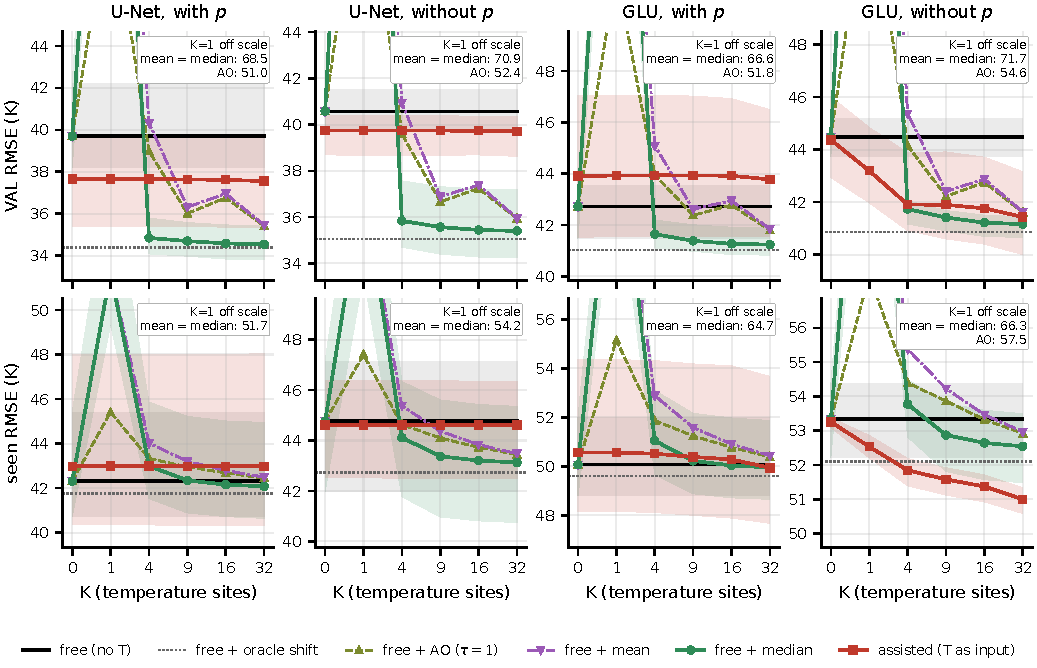
\includegraphics[width=\textwidth]{figures/month2/rmse_vs_K.pdf}
  \caption{Common-domain macro RMSE versus the number $K$ of temperature sites, best checkpoints, 5\% velocity (top: VAL; bottom: seen). Each curve is the mean over three seeds of the mean over three layout/mask pairs. Shaded bands show the seed range for the free model, the median correction and the temperature-input model. The dotted line is the oracle uniform shift (diagnostic). The free model and the corrections use the same frozen network. The temperature-input (\emph{assisted}) curve is a separately trained network (Section~\ref{sec:assisted}). Values at $K{=}1$ outside the axis range are printed in each panel.}
  \label{fig:K}
\end{figure}

\begin{table}[!htb]
\centering
\caption{Common-domain macro RMSE (K), best checkpoints, 5\% velocity, mean over three seeds and three layout/mask pairs. ``Assisted'' columns refer to the separately trained temperature-input models of Section~\ref{sec:assisted}. $\Delta$ = assisted($K{=}32$) $-$ assisted($K{=}0$), the gain attributable to the temperatures within the same model.}
\label{tab:joint}
\footnotesize
\setlength{\tabcolsep}{3.5pt}
\begin{tabular}{llrrrrrrrrr}
\toprule
 & & free & mean & \multicolumn{2}{c}{median} & AO & oracle & \multicolumn{3}{c}{assisted} \\
\cmidrule(lr){5-6}\cmidrule(lr){9-11}
Model & $\mathbf{p}$ & & $K{=}1$ & $K{=}4$ & $K{=}32$ & $K{=}32$ & shift & $K{=}0$ & $K{=}32$ & $\Delta$ \\
\midrule
\tabinput{tables/month2/joint_main.tex}
\bottomrule
\end{tabular}
\end{table}

\textbf{The median corrects the level once $K\ge4$.} For the U-Net \pon\ on VAL (Figure~\ref{fig:K}, Table~\ref{tab:joint}), the median lowers the error from $39.70$ to $34.85\K$ at $K{=}4$, then to $34.69$, $34.58$ and $34.54\K$ at $K{=}9$, $16$, $32$. The oracle shift gives $34.38\K$. Thus $94\%$ of the gain available at $K{=}32$ is already obtained at $K{=}4$, and later sites add only $0.31\K$. The U-Net \poff\ behaves the same way ($40.57\to35.84\to35.40\K$). For the GLU the gain is smaller, because its level was already better: $42.72\to41.24\K$ (\pon) and $44.48\to41.16\K$ (\poff) at $K{=}32$. The median also narrows the seed spread of the U-Net \pon\ from $4.0$ to $1.6\K$ at $K{=}32$. For every $K\ge4$, none of the 36 neural cells (configuration $\times$ seed $\times$ layout) is worse than the free model on VAL. The gain is concentrated in \cond{40}{0.90}: for the U-Net \pon\ it falls from $38.4$ to $24.0\K$, with smaller or no change elsewhere (Table~\ref{tab:condK}). Once the level is corrected, the advantage of the U-Net \pon\ over the GLU \pon\ grows from about $3\K$ to $6.7\K$ on VAL, with disjoint seed ranges. This is the structural gap of Section~\ref{sec:families} made visible.

\textbf{The mean and the shrunk mean are fragile.} Both react strongly to sites falling in the jets. On VAL, the mean is worse than the free model in 12 of 36 neural cells at $K{=}4$, and still in 11 at $K{=}16$. Its curve is not monotonic because new sites added between $K{=}9$ and $K{=}16$ in one layout lie in the upper jet. Shrinkage ($\tau{=}1$) changes little once $K$ is large. The advantage of the median comes from robustness to jet outliers, not from removing the shrinkage.

\begin{figure}[!htb]
  \centering
  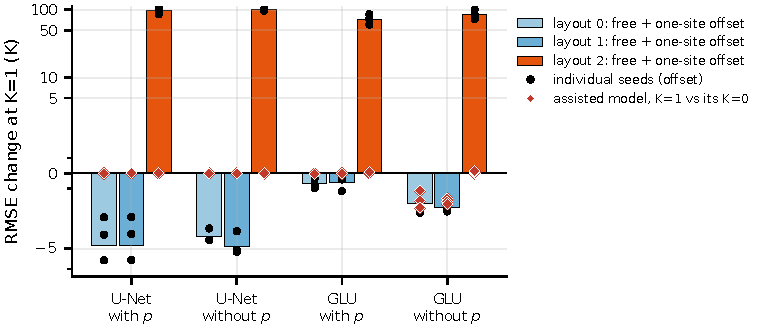
\includegraphics[width=0.8\textwidth]{figures/month2/k1_by_layout.pdf}
  \caption{Change of VAL common-domain RMSE at $K{=}1$ with respect to the free model, separately for each layout/mask pair, best checkpoints (symmetric-log axis). Bars: seed mean of the single-site offset (mean = median at $K{=}1$); black dots: individual seeds. Red diamonds: temperature-input model at $K{=}1$ minus the same model at $K{=}0$ (one per seed).}
  \label{fig:k1}
\end{figure}

\textbf{One site is unsafe, and the failure comes from one layout.} At $K{=}1$, the average VAL error rises to $66.6$--$71.7\K$ for all four configurations. Figure~\ref{fig:k1} shows that this average hides two different behaviours. In layouts 0 and 1 the single site lies in the hot region, and the correction \emph{improves} every model and seed (U-Net by $2.9$--$7.4\K$, GLU by $0.3$--$2.6\K$). In layout~2 the site lies in the lower cold jet (Figure~\ref{fig:layouts}). There, the local residual of hundreds of kelvin is shifted onto the whole field, and the U-Net \pon\ error rises from $39.7$ to $135.7\K$. A single site therefore carries a large risk that depends on its position, so one point measurement should not be used as a uniform offset.

\textbf{On seen frames the median gives little or nothing at small $K$.} On seen frames the free \pon\ models already have a small level error: the oracle would gain only $0.6\K$ for the U-Net. Here the median at $K{=}4$ \emph{worsens} the average for three of four configurations (U-Net \pon\ $42.32\to42.99\K$, GLU \pon\ $50.06\to51.04\K$). Only at $K{=}32$ is no neural model (any seed or layout) worse than its free prediction. Whether a few temperatures help depends on how large the level error is compared with the noise of the offset estimate. The VAL saturation at $K{=}4$ is therefore not a general sensor count.

\textbf{Structure is unchanged, and jets may get worse.} After the median correction at $K{=}32$ on VAL, the hot-region RMSE of the U-Net \pon\ drops from $21.6$ to $13.1\K$, while the jet RMSE stays at about $114$--$116\K$ (Table~\ref{tab:regional}). A uniform shift that fits the hot majority of the field moves the cold minority in the wrong direction. Improving the global metric can therefore worsen one region.

\textbf{A joint linear solve can use temperatures for structure.} The GappyPOD baseline offers a useful contrast (Table~\ref{tab:baseK} in the appendix). When the $K$ temperatures enter the modal least-squares solve as extra rows (T-block), the VAL error at $K{=}32$ reaches $64.0\K$ (\pon) and $64.7\K$ (\poff). This is \emph{below} the oracle uniform shift of the same model ($68.2$ and $70.3\K$). Point temperatures can therefore also correct spatial structure when the reconstruction lets them change spatial degrees of freedom. GappyPOD nevertheless remains far above the neural models.

\keybox{\textbf{Supported (within the tested layouts, ideal temperatures, VAL and seen).} The median of $K\ge4$ residuals corrects most of the level error of the temperature-free networks, with no VAL degradation for the neural models. It leaves structure unchanged. A single site is unreliable and its effect depends on position.
\textbf{Not supported.} That ``four thermocouples suffice''. The saturation at $K{=}4$ reflects three VAL conditions, three random layouts and noise-free values. On seen frames, small $K$ does not help.}

%======================================================================
\section{Temperatures as network input}
\label{sec:assisted}

\subsection{Why a different experiment}

A post hoc correction can only shift the field. A network that receives the temperatures as input could in principle also correct the jets and flame position, or ignore a misleading site. We trained twelve new models to test this. They use the same families, $\mathbf{p}$ settings and seeds as Experiment~1, and the same data, velocity observations, $K$ values and evaluation sites as Experiment~2. The temperature values and their positions are actually provided to the network:
\begin{itemize}
  \item the U-Net receives two extra input channels (normalized temperature at the observed sites and a temperature mask);
  \item the GLU receives typed temperature tokens alongside the velocity tokens.
\end{itemize}
A single model per configuration is trained with $K$ drawn for each batch uniformly from the six values $\{0,1,4,9,16,32\}$, at random training sites. The best checkpoint minimizes the VAL error averaged over the six $K$, a different criterion from Experiment~1. The GLU here also uses an exact lattice neighbour search, which differs slightly from the temperature-free GLU.

Two consequences follow for reading the results. First, at $K{=}0$ the new model is \emph{not} the model of Experiment~1: it is a separate training, with different initialization of the input layer, a different selection criterion and different epochs. Second, the only clean measure of what the temperatures contribute is the change of the same model between $K{=}0$ and $K>0$. Any difference between the new model at $K{=}0$ and the free model reflects training variability, not the temperatures.

\subsection{Results}

\begin{figure}[!htb]
  \centering
  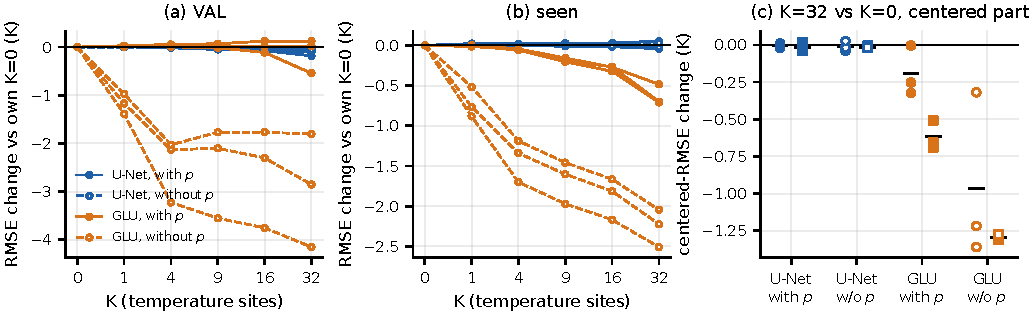
\includegraphics[width=\textwidth]{figures/month2/assisted_gain.pdf}
  \caption{Temperature-input models: change of common-domain RMSE with respect to the same model at $K{=}0$, best checkpoints, one line per training seed (mean of three layout/mask pairs). (a)~VAL; (b)~seen. (c)~Change of the centered RMSE (structural part) between $K{=}32$ and $K{=}0$: circles VAL, squares seen, one marker per seed, bars at the seed mean. Filled/solid: \pon; open/dashed: \poff.}
  \label{fig:gain}
\end{figure}

\textbf{Within-model gains are small except for one configuration} (Figure~\ref{fig:gain}, Table~\ref{tab:joint}).
\begin{itemize}
  \item \emph{U-Net, both settings.} The gain from $K{=}0$ to $K{=}32$ is $-0.10\K$ (\pon, seed range $-0.18$ to $-0.03$) and $-0.03\K$ (\poff) on VAL, and essentially zero on seen frames. The centered RMSE does not change. The same holds at the last checkpoint, after more than 600 epochs.
  \item \emph{GLU \pon.} The gain is $-0.13\K$ on VAL. On seen frames it is a consistent $-0.63\K$ across all three seeds, almost entirely structural.
  \item \emph{GLU \poff.} This is the one configuration with a clear benefit. It improves in all three seeds, already at $K{=}1$ ($-1.18\K$) and at $K{=}4$ ($-2.46\K$), reaching $-2.94\K$ at $K{=}32$ on VAL (seed range $-4.15$ to $-1.81$) and $-2.26\K$ on seen. The gain is mainly in the level. The VAL signed bias moves from $-4.6$ to $+2.0\K$ and the hot-region RMSE from $26.9$ to $21.1\K$. It is also partly structural: centered RMSE falls by $0.97\K$ on VAL and $1.29\K$ on seen.
\end{itemize}
In the jet layout at $K{=}1$ the GLU \poff\ is essentially unaffected ($+0.08\K$), whereas the single-site offset adds $86\K$ (Figure~\ref{fig:k1}). This does not show that the network has learned to recognize outliers. It shows only that this model did not transfer that site's residual to the whole field.

\textbf{Do not attribute the $K{=}0$ difference to the temperatures.} On VAL, the U-Net \pon\ trained with temperature input scores $37.66\K$ at $K{=}0$, against $39.70\K$ for the free model. This advantage is already present without any temperature. It comes mostly from one seed, where the free run was the worst ($42.2\K$) and the new run the best ($35.4\K$). The differences at $K{=}0$ range from $-6.8$ to $+3.5\K$ across runs, in both directions. On seen frames the new U-Net \pon\ is $0.7\K$ worse at $K{=}0$.

\textbf{Comparison with the free model plus median.} On VAL at $K\ge4$, the free model with the median correction is lower than the temperature-input model on average in all four configurations. At $K{=}32$ the values are $34.54$ vs $37.55\K$ (U-Net \pon), $35.40$ vs $39.71\K$ (U-Net \poff), $41.24$ vs $43.78\K$ (GLU \pon) and $41.16$ vs $41.43\K$ (GLU \poff). This holds for every seed except two seeds of the GLU \poff, where the temperature-input model is slightly better. On seen frames the GLU \poff\ with temperature input ($51.00\K$) is lower than its free-plus-median counterpart ($52.54\K$) in all three seeds, and even below the oracle shift ($52.09\K$). It remains about $9\K$ above the U-Net. These comparisons mix model differences and use of the sites, so they are descriptive.

\textbf{What we cannot conclude.} The small gains do not show that the networks ignore the temperature values, or that a U-Net cannot assimilate them. A small positive control before the campaign confirmed that both networks can read the temperature inputs. We did not perform a controlled perturbation of the input temperatures on the trained models. Several mechanisms could limit the use of the temperatures:
\begin{itemize}
  \item the loss weight of 32 sites among 16384 pixels (0.2\%);
  \item smoothing of single-pixel inputs by convolutions and normalization;
  \item partial redundancy between $\mathbf{p}$ and the temperatures for the level;
  \item the choice of $K$ distribution in training.
\end{itemize}
None of these was isolated, and we do not attribute the result to any of them.

The plan foresaw a simple spatial interpolation of the residuals (kernel or RBF fitted on training data) as a baseline for any learned spatial correction. It was \textbf{not run}. Since the temperature-input models did not beat the median correction, there was no learned spatial gain to qualify. The omission still means we have not tested how much spatial information beyond the level a simple interpolation of the residuals could extract. This baseline is the first step of direction~C in Section~\ref{sec:month3}.

\keybox{\textbf{Supported.} In the tested recipe (uniform full-field loss, $K$ uniform over six values, training from scratch), temperature input gave a negligible within-model gain for three configurations. It gave a measurable level and modest structural gain for the GLU \poff, which was also robust to the jet site at $K{=}1$. On VAL it did not beat the median correction of the free models on average.
\textbf{Open.} Whether a formulation that reads the residuals explicitly, or a different loss, could recover structural information from few sites.}

%======================================================================
\section{Synthesis of Month 2 and limits}
\label{sec:synthesis}

\textbf{What has been shown, within the tested perimeter.}
\begin{enumerate}
  \item A single sparse velocity snapshot (5\%, two components) supports a neural temperature reconstruction with 1.6 to 2.5 times lower error than the linear GappyPOD baseline on held-out VAL conditions and on later frames of training conditions. The predictions depend on the observed instant. Training-data quantity matters, mainly for structure.
  \item The remaining error has two parts that respond to different remedies:
  \begin{itemize}
    \item a \emph{level} part, concentrated in some held-out conditions, which a robust offset from $K\ge4$ ideal temperatures largely removes;
    \item a \emph{structural} part, dominated by the cold jets, which no uniform correction touches.
  \end{itemize}
  \item The two families trade these parts differently: the U-Net has the better structure, the GLU the better level and lower sensitivity to velocity density.
  \item Feeding temperatures to the network, in the tested recipe, did not add much beyond the offset, except for the GLU \poff.
\end{enumerate}

\textbf{Provisional operating reference and preserved alternatives.} For subsequent work, we use the U-Net \pon\ trained without temperatures at 5\% velocity as the working reference (U-Net \poff\ when $\mathbf{p}$ is not available), and the same model plus the median offset when $K\ge4$ ideal temperatures are available. This is a post-results development choice. It was not pre-registered, it is not a claim of architectural superiority, and it does not guarantee improvement in every condition. The following remain documented alternatives:
\begin{itemize}
  \item the GLU, which has a better level and better tolerance to other densities;
  \item the GLU \poff\ with temperature input, the only configuration with a measurable within-model use of temperatures;
  \item GappyPOD with the T-block, a linear reference that shows that temperatures can also correct structure.
\end{itemize}

\textbf{What we cannot conclude.}
\begin{itemize}
  \item \emph{Generalization.} Three VAL conditions, used for selection, scheduling, stopping and for choosing the median, cannot establish generalization to new operating conditions. No TEST data were used, and the Month~1 baselines had already been evaluated on the TEST conditions.
  \item \emph{Measurement realism.} Ideal noise-free temperatures and random point layouts do not validate thermocouples, which have noise, response lag, intrusiveness and placement limits. Nor do they establish a required number of sensors.
  \item \emph{Variability.} Three seeds give a descriptive range, not a robust distribution. Each pair of temperature layout and velocity mask varies jointly.
  \item \emph{Architecture.} The U-Net/GLU comparison concerns two specific recipes with different capacities (4.90\,M vs 1.15\,M parameters) and implementations.
  \item \emph{Temperature use.} Small gains from temperature input do not prove that the information is absent or unusable.
\end{itemize}

\textbf{Cost.} Table~\ref{tab:costs} lists measured compute and queue times. In the temperature-free campaign, training took $3.7$--$4.2$\,h per U-Net run and $5.5$--$7.8$\,h per GLU run. The temperature-input campaign was faster: $0.6$--$0.8$\,h for the U-Net and $2.4$--$3.4$\,h for the GLU. The two campaigns differ in implementation and in compute partition, so these numbers do not define a fixed cost ratio between the families.

%======================================================================
\section{Proposed next steps and connection to realistic applications}
\label{sec:month3}

Month~2 leaves two clearly separated problems: the structural error in the jets and a level error whose generality is unknown. It also leaves an open question about how few temperatures can best be used. I propose to use the U-Net \pon\ as the working reference and to investigate the following three directions within a bounded program. The residual-assimilation study keeps the backbone frozen; the jet-loss and condition-fold studies require retraining controlled variants. The aim is to identify which improvements survive changes in conditions and observations, while defining a concrete application with domain-expert input. The final scope of that application is still being developed.

\subsection*{A. Better reconstruction of the jets without temperature}
\begin{itemize}
  \item \textbf{Question.} Does a training loss that gives more weight to errors in the cold jets improve the structure of the temperature-free reconstruction without degrading the rest of the field?
  \item \textbf{Design.} A single loss variant of the same U-Net, data, observations, seeds and checkpoint rule. It adds a weighted term on the training pixels with true $T<1800\K$, with the weight fixed before training. The true temperature enters only the training loss; at inference the task remains temperature-free.
  \item \textbf{Evaluation.} Jet RMSE (with and without removing the frame bias), global and centered RMSE, the hot region, and each condition separately.
  \item \textbf{Expected benefit.} It acts on the structural residual that an offset cannot correct.
  \item \textbf{Risks.} The method may specialize to the chosen threshold, region or dataset, and it may trade accuracy in the hot regions or in the global error for the jets. Whether this happens must be measured, ideally within a generalization check. It is a risk to verify, not an established overfitting.
\end{itemize}

\subsection*{B. Does the thermal-level error generalize?}
\begin{itemize}
  \item \textbf{Question.} On operating conditions excluded from training, is the level error systematic and predictable from $\mathbf{p}$ or velocity, or does the current evidence rest on one or two VAL cases (mainly \cond{40}{0.90})?
  \item \textbf{Design.} Measure the bias on further held-out conditions with a frozen protocol \emph{before} designing any remedy. Two options exist:
  \begin{itemize}
    \item leave-condition-out folds within the TRAIN conditions, which require retraining with fold-specific normalisation and priors. Two geometrically extrapolative candidates were identified, \cond{40}{0.85} and \cond{80}{1.20}, but are not fixed.
    \item a separately agreed evaluation on data that has not been used for selection.
  \end{itemize}
  I will define the evaluation design before running it, taking account of which conditions have already informed development. Any use of TEST data will be documented separately rather than treated as an untouched confirmation by default.
  \item \textbf{Expected benefit.} It distinguishes a systematic problem from a few VAL cases, and it reduces the risk of further optimizing the method on the three VAL conditions already used.
  \item \textbf{Cost and limits.} Folds require training, and the independence of each evaluation set must be defined precisely given the history of the data. A single biased case would not establish a general law. Conversely, if the bias proves unpredictable, this would not prove that thermal measurements are indispensable.
\end{itemize}

\subsection*{C. Spatial assimilation of temperature residuals on a frozen network}
\begin{itemize}
  \item \textbf{Question.} Can a few temperatures correct structure, and not only level, if they are used explicitly as residuals of the temperature-free prediction?
  \item \textbf{Design.} The frozen U-Net produces the field. At each observed site we compute $r_k=T_{\text{obs}}(\mathbf{x}_k)-\hat T_{\text{free}}(\mathbf{x}_k)$. A corrector maps residuals and coordinates (possibly with snapshot context) to a spatial correction map, which is exactly zero at $K{=}0$. The method thus differs both from the median, which produces a single offset, and from the training of Section~\ref{sec:assisted}, which received raw temperatures and could change the base reconstruction.
  \item \textbf{Steps.} First, an inexpensive spatial baseline (RBF/kernel interpolation or a POD of the residuals, fitted on training data, same $K$ and layouts). Then, if warranted, a single learned residual module trained with three seeds and compared against the free model, the free model plus median and that baseline. The evaluation covers the common domain, centered RMSE, jets, hot region, seen frames and each condition.
  \item \textbf{Expected benefit.} It separates the quality of the backbone from the assimilation of measurements and tests whether gains beyond the median exist. It also connects naturally to variable sensor numbers and layouts.
  \item \textbf{Risks.} An apparent advantage might come from simple interpolation. Residuals on training frames, where the backbone is well fitted, may be much smaller and differently distributed than on new conditions. Robustness to layout and noise is untested, and exact consistency with noisy measurements would require an uncertainty model. A failure would not prove that a few temperatures contain no structural information.
\end{itemize}

\subsection*{How the directions relate, and a possible ordered program}

The three directions are not mutually exclusive. A generalization check (B) is also the natural way to evaluate the two methodological changes (A and C), because it tests them on conditions that played no role in their design. Training is relatively fast: a U-Net run took about 4\,h in the temperature-free campaign and under 1\,h in the temperature-input campaign, and the campaigns ran up to four jobs concurrently. It would therefore be feasible to address all three directions in one bounded program rather than choosing only one. I therefore see scope to pursue all three through a small, ordered set of experiments while the application requirements are being clarified, rather than committing immediately to a large campaign.

Computation is not the main constraint. Analysis takes time, and every new decision made on the same three VAL conditions makes them less informative. I propose the following sequence with explicit decision points:
\begin{enumerate}
  \item \textbf{Freeze first.} Specify the generalization design for B, the evaluation metrics and the success criteria for A and C, and the single loss weight for A, all before any new result is seen.
  \item \textbf{Inexpensive steps.} Run the spatial residual baseline of C. It needs no network training but requires inference of the frozen model on training frames, whose cost has not yet been profiled. In parallel, launch the trainings of A (three seeds) and the folds of B once their evaluation design is fixed. Their cost per run is expected to be comparable to the measured U-Net runs above, multiplied by the number of folds and seeds. \emph{Decision point:} continue C with a learned module only if the baseline shows a structural gain beyond the median, or if the comparison remains inconclusive.
  \item \textbf{Joint evaluation.} Evaluate the jet-weighted model and, if trained, the residual module under the frozen generalization protocol, against the unchanged reference. The cost of a learned residual module has not been profiled, and we do not estimate it here.
\end{enumerate}

The thesis question remains general: reconstruction of a single instantaneous field from incomplete observations, under changes in the number and position of sensors, measurement noise, physical constraints and, if possible, the dataset. Month~3 should therefore not become an optimization of the three current VAL conditions. Noise and realistic sensor layouts are natural axes for later months. Which of them are central to the thesis should be decided explicitly, not added as an open list.

\subsection*{Connecting the benchmark to a realistic measurement problem}

The next stage should establish where this reconstruction framework could answer a useful experimental or engineering question. As previously discussed with my MIT supervisor, I am seeking input from my Politecnico di Milano supervisor on a concrete combustion or engine application. I plan to arrange a discussion about which quantities are genuinely inaccessible, what velocity and temperature measurements can be acquired together, and where temperature sensors can physically be placed. Suitable engine datasets or experimental measurements, if available, could provide a more relevant setting in which to test transfer beyond the present numerical benchmark. Access to such data has not yet been established.

This domain input will help define meaningful sensor layouts, measurement uncertainty, response times and other physical constraints. These requirements should shape the next application rather than be added only after optimizing a method on the current VAL conditions. In the meantime, the controlled studies above can clarify the limitations of the existing reconstruction framework without depending on access to a new dataset.

The current results support instantaneous reconstruction on this numerical benchmark: neural models substantially outperform the baselines, and the snapshot-swap tests show dependence on the observed instant. The remaining risk is how much of that capability transfers to realistic observations and different operating conditions. Alongside improving accuracy, I will develop a fallback contribution based on quantifying the conditions under which reconstruction is reliable, which observations are informative, and where the available measurements leave substantial ambiguity. This would require a carefully defined evaluation; the current experiments do not establish an irreducible physical limit.

I welcome feedback on the physical relevance of these proposed studies and on suitable application settings. I will use that input, together with the domain-expert discussion, to refine the scope and evaluation of the next stage.

%======================================================================
\clearpage
\appendix
\section{Run matrix and checkpoint criteria}
\label{app:runs}

\begin{table}[H]
\centering
\caption{The 24 trainings of Experiments~1 and~3 (149-frame pool, 5\% velocity). All stopped by the plateau criterion. ``Best'' is the first VAL minimum (Experiment~1: VAL error at 5\%; Experiment~3: VAL error averaged over the six $K$). ``Last'' is the epoch at early stop. Compute is GPU time in hours from the scheduler accounting. $^\dagger$Reused from the data-quantity study after verifying files and hashes. $^\ddagger$Continued from epoch 1000 with unchanged rules until the plateau criterion was met. The best epoch did not change.}
\label{tab:runs}
\footnotesize
\begin{tabular}{lllcrrrrrrr}
\toprule
 & & & \multicolumn{4}{c}{\textbf{Exp.~1: temperature-free}} & \multicolumn{4}{c}{\textbf{Exp.~3: temperature input}} \\
\cmidrule(lr){4-7}\cmidrule(lr){8-11}
Model & $\mathbf{p}$ & seed & run & best & last & h & best & last & attempts & h \\
\midrule
\tabinput{tables/month2/run_matrix.tex}
\bottomrule
\end{tabular}
\end{table}

Training repeated attempts only after scheduler preemption or time limits. Each resumed from the complete saved state of the same run, never from scratch. In Experiment~3, three GLU runs had reached the initial limit of 1000 epochs without meeting the plateau criterion. They were continued with unchanged rules and stopped at epochs 1030, 1080 and 1060. Their best checkpoints did not change. Only the last-checkpoint values moved, by $0.04$--$0.46\K$. Values in this report use the final state.

%----------------------------------------------------------------------
\section{Protocol, metrics and domains}
\label{app:protocol}

\textbf{Frames.} Each condition has 2001 frames at $\Delta t=0.25$\,ms. The frame sets are:
\begin{itemize}
  \item training pool: frames 0--1480 every 10 frames (149 per TRAIN condition);
  \item fit reference and normalisation: frames 0--1480 every 40 frames (38 per condition, 760 in total);
  \item seen: frames 1600--2000 every 40 frames (11 per TRAIN condition);
  \item VAL: frames 0--2000 every 50 frames (41 per condition).
\end{itemize}
The 19- and 38-frame pools of the data-quantity study are nested subsets of the 149-frame pool. The data-quantity study kept the number of optimizer updates per epoch fixed (760 presentations, 95 updates of batch 8).

\textbf{Inputs.}
\begin{itemize}
  \item U-Net: normalized $v_i,v_j$ at observed sites (zero elsewhere), a binary observation mask, two coordinates, and normalized $(\NH\%,\phi)$ as constant channels, which are set to zero \poff.
  \item GLU: one token per observed site with isotropically scaled coordinates and velocity; $\mathbf{p}$ is added through a bias-free projection.
  \item Temperature-input variants: U-Net with two more channels (normalized temperature and temperature mask); GLU with typed temperature tokens.
\end{itemize}

\textbf{Optimization.} The settings are:
\begin{itemize}
  \item AdamW (learning rate $10^{-3}$, weight decay $10^{-4}$), gradient clipping at norm 1, fp32;
  \item warm-up of 950 updates, then a plateau scheduler on the VAL error (factor 0.5, patience 5 evaluations, minimum $10^{-5}$);
  \item evaluation every 10 epochs, early stopping after at least 200 epochs and 15 evaluations without 0.1\% relative improvement;
  \item an initial tranche of 1000 epochs, which may be extended with unchanged rules.
\end{itemize}

\textbf{Metrics.} A macro value is computed as a per-frame metric, averaged over the frames of a condition, then uniformly over conditions (3 for VAL, 20 for seen), then over the three mask replicas. Seed statistics (mean, minimum, maximum) are computed last. The bias is mean(prediction $-$ truth). The centered RMSE is the RMSE after subtracting the frame's own bias. The fixed regions are hot ($T\ge2100\K$), peak ($T\ge2200\K$) and jets ($T<1800\K$). The hot-region IoU uses $T\ge2100\K$. Regional values are full-field regions defined on the true field.

\textbf{Domains for the temperature experiments.}
\begin{itemize}
  \item Full field: 16384 pixels.
  \item Common domain: the grid minus the 32 sites of the layout, 16352 pixels for every $K$. This is the primary domain for comparisons across $K$.
  \item Off-anchor($K$): the grid minus the first $K$ sites.
  \item Anchors: the $K$ observed sites.
\end{itemize}
Values from different domains are never mixed in one comparison. For the temperature-input models, off-anchor and common-domain values agree within $0.1\K$.

\textbf{Baselines (149-frame pool).} The global mean and the parametric mean field (piecewise-linear in $\phi$) are fitted once. GappyPOD uses $R{=}32$ joint velocity--temperature modes with the regularization fixed in Month~1. The same code reproduces the historical 38-frame baselines to within $2.5\times10^{-8}\K$, and refitting on 149 frames changes the VAL values by at most $1\K$. The T-block adds the $K$ temperature rows to the modal solve with the historical weights.

%----------------------------------------------------------------------
\section{Extended tables}
\label{app:tables}

\begin{table}[H]
\centering
\caption{Temperature-free models, individual seeds (best checkpoint, 5\% velocity unless stated; mean of three mask replicas; errors in K). Stop = epoch at early stop. ``fit ref.'' = 760 training frames.}
\label{tab:seeds}
\footnotesize
\setlength{\tabcolsep}{3.2pt}
\begin{tabular}{llcrrrrrrrrrr}
\toprule
 & & & \multicolumn{2}{c}{epoch} & \multicolumn{4}{c}{VAL 5\%} & seen & fit ref. & \multicolumn{2}{c}{VAL RMSE} \\
\cmidrule(lr){4-5}\cmidrule(lr){6-9}\cmidrule(lr){12-13}
Model & $\mathbf{p}$ & seed & best & stop & RMSE & centered & bias & IoU & RMSE & RMSE & 1\% & 20\% \\
\midrule
\tabinput{tables/month2/free_per_seed.tex}
\bottomrule
\end{tabular}
\end{table}

\begin{table}[H]
\centering
\caption{Temperature-free models per VAL condition (full field, best checkpoint, 5\% velocity, mean over three seeds; signed bias with the seed range).}
\label{tab:freecond}
\footnotesize
\setlength{\tabcolsep}{2.6pt}
\begin{tabular}{llrrrrrrrrrrrr}
\toprule
 & & \multicolumn{4}{c}{\cond{0}{1.05}} & \multicolumn{4}{c}{\cond{20}{1.10}} & \multicolumn{4}{c}{\cond{40}{0.90}} \\
\cmidrule(lr){3-6}\cmidrule(lr){7-10}\cmidrule(lr){11-14}
Model & $\mathbf{p}$ & RMSE & bias & jets & IoU & RMSE & bias & jets & IoU & RMSE & bias & jets & IoU \\
\midrule
\tabinput{tables/month2/free_per_condition.tex}
\bottomrule
\end{tabular}
\end{table}

\begin{table}[H]
\centering
\caption{Per-condition common-domain RMSE on VAL (best checkpoint, mean over three seeds and three layout/mask pairs): free model, free model plus median at $K{=}4$ and $K{=}32$, and the temperature-input model at $K{=}0$ and $K{=}32$.}
\label{tab:condK}
\footnotesize
\setlength{\tabcolsep}{2.3pt}
\begin{tabular}{llrrrrrrrrrrrrrrr}
\toprule
 & & \multicolumn{5}{c}{\cond{0}{1.05}} & \multicolumn{5}{c}{\cond{20}{1.10}} & \multicolumn{5}{c}{\cond{40}{0.90}} \\
\cmidrule(lr){3-7}\cmidrule(lr){8-12}\cmidrule(lr){13-17}
 & & free & \multicolumn{2}{c}{median} & \multicolumn{2}{c}{input} & free & \multicolumn{2}{c}{median} & \multicolumn{2}{c}{input} & free & \multicolumn{2}{c}{median} & \multicolumn{2}{c}{input} \\
Model & $\mathbf{p}$ & & 4 & 32 & 0 & 32 & & 4 & 32 & 0 & 32 & & 4 & 32 & 0 & 32 \\
\midrule
\tabinput{tables/month2/per_condition_K.tex}
\bottomrule
\end{tabular}
\end{table}

\begin{table}[H]
\centering
\caption{Regional errors on VAL (full-field regions, best checkpoint, mean over three seeds and layout/mask pairs). Free = temperature-free model; med32 = free + median at $K{=}32$; in0 and in32 = temperature-input model at $K{=}0$ and $K{=}32$. The median leaves the centered RMSE unchanged by construction.}
\label{tab:regional}
\footnotesize
\setlength{\tabcolsep}{2.8pt}
\begin{tabular}{llrrrrrrrrrrrr}
\toprule
 & & \multicolumn{4}{c}{hot region RMSE} & \multicolumn{4}{c}{jet RMSE ($T<1800\K$)} & \multicolumn{4}{c}{centered RMSE} \\
\cmidrule(lr){3-6}\cmidrule(lr){7-10}\cmidrule(lr){11-14}
Model & $\mathbf{p}$ & free & med32 & in0 & in32 & free & med32 & in0 & in32 & free & med32 & in0 & in32 \\
\midrule
\tabinput{tables/month2/regional_K32.tex}
\bottomrule
\end{tabular}
\end{table}

\begin{table}[H]
\centering
\caption{Baselines with temperature sites: common-domain RMSE versus $K$ (fitted once on the 149-frame pool; mean of three layout/mask pairs). The T-block solves for the POD coefficients with the temperature rows. The last column is the oracle uniform shift of the free baseline.}
\label{tab:baseK}
\footnotesize
\begin{tabular}{lrrrrrrr}
\toprule
Method & $K{=}0$ & 1 & 4 & 9 & 16 & 32 & oracle \\
\midrule
\tabinput{tables/month2/baselines_K.tex}
\bottomrule
\end{tabular}
\end{table}

%----------------------------------------------------------------------
\section{Costs and provenance}
\label{app:costs}

\begin{table}[H]
\centering
\caption{Training cost per run (hours, range over runs) from the scheduler accounting. Compute is the time the job ran on a GPU. Queue is the waiting time, and for the temperature-free GLU array it includes a cap of four concurrent tasks. Attempts above one are resumptions after preemption or time limits. Temperature-input GLU runs used a preemptable partition. Final evaluation took 53--82\,min per run in Experiment~1 (81 evaluation settings per run).}
\label{tab:costs}
\small
\begin{tabular}{llrrrr}
\toprule
Campaign & Model & runs & compute (h) & queue (h) & attempts \\
\midrule
\tabinput{tables/month2/costs.tex}
\bottomrule
\end{tabular}
\end{table}

\textbf{Provenance.} All results come from versioned tables in the project repository \nolinkurl{EnricoBontempi/official_thesis}. The commits are:
\begin{itemize}
  \item temperature-free comparison: \texttt{2879c1b};
  \item correction sweep: \texttt{be18ad0};
  \item temperature-input study (final version, including the three continued runs) and joint comparison: \texttt{d20232e};
  \item data-quantity study: \texttt{4f0e263}.
\end{itemize}
The figures and table bodies of this report are regenerated from copies of those tables by \nolinkurl{month2_sources/make_figures.py}, without new evaluation. \nolinkurl{month2_sources/SOURCES.md} maps each figure and table to its source file and commit. \nolinkurl{month2_sources/NUMBERS.md} lists every quoted value with its source. Figure~\ref{fig:fields} is a crop of a published field figure. The level-versus-structure history quoted in Sections~\ref{sec:objective} and~\ref{sec:correction} (38-frame models, nine-site grid) and the dense diagnostic come from the corresponding project reports.

%----------------------------------------------------------------------
\section{Technical notes for reproducibility}
\label{app:notes}

\begin{itemize}
  \item \textbf{Verification gates.} Every evaluation was checked against the values logged during training (tolerance $0.05\K$ on macro RMSE). The recorded maximum deviation was $0\K$. The temperature-free reference of the correction sweep reproduces the Experiment~1 per-frame values exactly. The joint comparison verified identical anchor manifest, $K$ values, layouts, frames, velocity-mask hashes (1029 frames) and macro definitions on both sides.
  \item \textbf{Protocol file erratum.} The common configuration file of the temperature study was frozen with a YAML syntax error at line~72 (unquoted text after a list) and cannot be parsed. The executed code used separate frozen manifests (sites, matrices) and recorded the protocol identity, and the cross-checks of the result tables found no numerical discrepancy attributable to the error. The frozen file is kept unchanged under its recorded hash. It must not be presented as a valid executable configuration. Any reuse requires a separate, corrected revision.
  \item \textbf{GLU neighbour ties.} On the regular grid, the top-$k$ neighbour search of the temperature-free GLU has distance ties that may be resolved differently when the batch shape changes. This moves a frame RMSE by at most $0.03$--$0.08\K$. All evaluations used the training batch shape. The temperature-input GLU uses an exact lattice search with a deterministic tie-break, one more reason to compare it only with its own $K{=}0$.
  \item \textbf{Undefined regions.} The peak region ($T\ge2200\K$) is empty in a few fit-reference frames. These are declared and excluded from regional means; global metrics have no missing values. Hot-region IoU was not computed in the correction and temperature-input tables, so improvements of the hot region are reported through its RMSE.
  \item \textbf{Not available.} High-percentile (e.g.\ 95th) frame errors cannot be reconstructed from the aggregate tables and are not reported. Per-frame CSV files and checkpoints are stored on the cluster with manifests and hashes and are not part of the repositories. The extension records of the three continued runs carry an empty last-epoch field in one manifest. The actual epochs (1030, 1080, 1060) are in the run summaries and in Table~\ref{tab:runs}.
\end{itemize}

\bibliographystyle{unsrt}
\bibliography{references}

\end{document}
